% tex file for normality
\par \indent The validity of our hypothesis tests for the estimated 
$\hat{\beta}$ values from the chosen linear regression model are largely 
dependent on whether we can reasonably assume that the errors in our model 
are independent and identically distributed from some normal distribution 
with mean zero and constant variance. We focus here on checking the normality 
assumption. It is generally wise to use visualizations, such as residual vs. 
fitted values plots and quantile-quantile plots to inspect residuals for 
patterns and abnormalities. However, considering the sheer quantity of data 
we are working with --- each of the 24 subjects has 64 $\times$ 64 $\times$ 34 
voxels that can each in turn be fitted to a model --- visual inspection is 
not practical. 

For this reason, we used the Shapiro-Wilk test for normality, 
which tests the null hypothesis that the data in question is normally 
distributed. A Shapiro-Wilk test was performed for each set of residuals 
corresponding to a single voxel's time course. That is, each test used around 
200 observations, or the number of time points for that particular subject. 
200 observations is not an especially large sample size, and for this reason, 
we express some concern because normality tests have low power for small 
sample sizes. Shapiro-Wilk may incorrectly fail to reject the null hypothesis 
due to this bias \cite{ghasemi2012normality}. 

The average proportion of Shaprio-Wilk test ``p-values'' above 0.05 was 0.742 
for the unmasked residuals across both subjects and voxels and noticeably 
lower at 0.630 for the masked residuals. However, since using the masked data 
is more theoretically justifiable (the unmasked data contains many voxels 
outside of the brain), we use the masked data for our analysis despite the 
lower proportion of voxels whose residuals meet our normality check. Note that 
these proportions suggest that only about two-thirds of the masked voxels have 
residuals that are approximately normal, and that the others deviate 
significantly from the normal distribution (especially when considering our 
concerns about the power of Shaprio-Wilk tests for small sample sizes). So when 
discussing our models and especially when looking at the conclusions made by 
our hypothesis tests, one should exercise caution about the validity of those 
conjectures. 

Figures \ref{fig:sw} and \ref{fig:sw_masked} compare the spatial distribution 
of the Shapiro-Wilk ``p-values'' for Subject 10's masked and unmasked data. 
The unmasked figure is very difficult to interpret, but the masked figure does 
suggest that while the spatial distribution of voxels with approximately 
normal residuals is reasonably uniform in many regions, there are a few areas 
that consistently have very low ``p-values'' at around or below the 0.05 
threshold. Examples of these regions for Subject 10 include a small area 
between the front and center of the brain and a few spots near the sides. 
However, these observations are not consistent across all subjects, so much 
of it may simply be due to noise. 

\begin{figure}[ht]
\centering
\begin{minipage}[b]{0.45\linewidth}
	\centering
	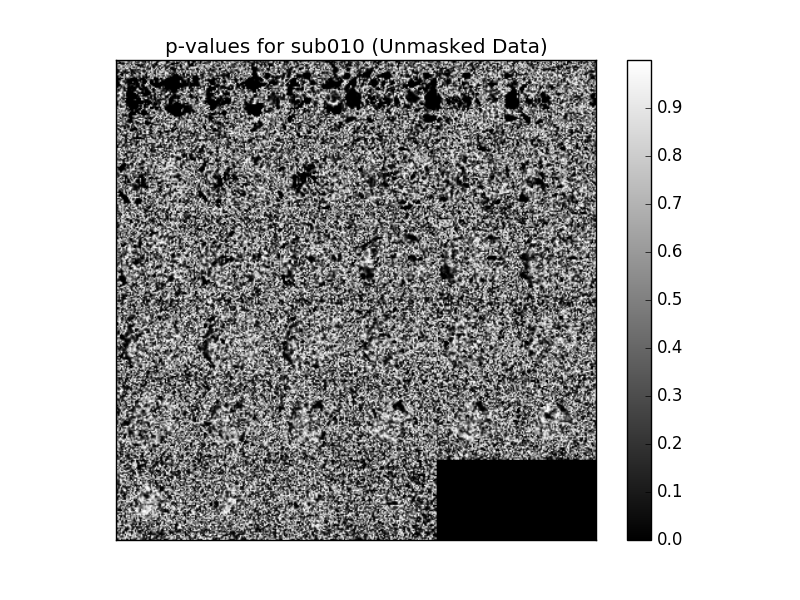
\includegraphics[width=.8\linewidth]{../images/sub010sw.png} 
	\caption{Subject 10's brain slices, with voxels colored by the magnitude of the
``p-value'' in the corresponding Shapiro-Wilk test for normality.Using unmasked residuals.}
\label{fig:sw}
\end{minipage}	
\quad
\begin{minipage}[b]{0.45\linewidth}
	\centering
		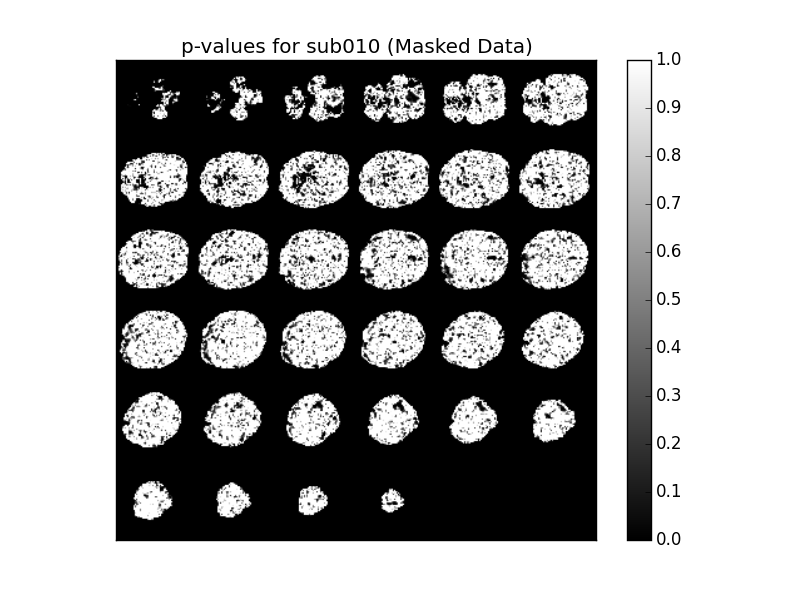
\includegraphics[width=.8\linewidth]{../images/sub010swmasked.png} 
	\caption{Subject 10's brain slices, with voxels colored by the magnitude of the
``p-value'' in the corresponding Shapiro-Wilk test for normality. Using masked residuals.}
\label{fig:sw_masked}
\end{minipage}
\end{figure}
